\documentclass{report}

\usepackage[margin=1in]{geometry}
\usepackage{amsmath,amssymb}
%\usepackage{dsfont} %install texlive-fonts-extra 
\usepackage{tikz}
\usetikzlibrary{bayesnet}

\author{Otto Fabius}
\title{SGVB Topic Modelling}
\begin{document}

\maketitle
\tableofcontents
\chapter{Introduction}

Generative modeling , neural nets in a few lines.

%A class of graphical models is that of Generative models, where the data in question is assumed to be generated by some process involving underlying factors (latent variables). 



\section{Variational Bayes}

Explain VB

\subsection{SGVB}

- General purpose introduction of sgvb . \\

- areas of success of sgvb.

\section{Bag-of-words Topic Modelling}
some paragraphs on (generative) topic modelling. 
Not too much detail but explain key idea and perhaps mention some pros and cons of current methods. 
\section{Research question}
Explain that we want to use sgvb for topic modelling. Introduce research question:
Can we perform large-scale, efficient, high-quality inference on bag-of-words representations of documents with sgvb? \\
Briefly discuss the advantages of this approach compared to other methods in topic modelling (one paragraph)
-	How do we deal with large vocabulary size?\\
-	What consequences do sparsity have/how can they be overcome? \\
-	What is learned in the (continuous) latent representation?



\pagebreak 
\nocite{*}
\bibliographystyle{amsplain}

\chapter{VAE Approach}
\section{Introduction}
In this Chapter we will elaborate on how we use a VAE approach for topic modeling. While we do not deviate conceptually from Kingma and Welling\cite{kingma2013auto}, we describe the full model to clarify the details w.r.t. topic modeling, as well as to explain some modeling choices.

\section{Method}

	
	The graphical model for such a VAE approach is as shown in Figure \ref{VAE}. When comparing this graphical model to e.g. LDA\cite{bleilda}, the largest difference is that this model only has one plate: each document is treated as an entity rather than a collection of words, and the model has document-level latent variables as opposed to word-level latent variables (mention DEF?). 
	
	\begin{figure}[ht]
		\begin{center}
			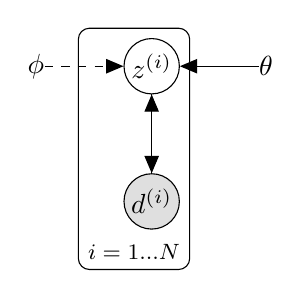
\begin{tikzpicture}[node distance = 1.5cm]
			
			
			\node[obs] (d) {$d^{(i)}$};
			
			\node[latent, above=of d] (z) {$z^{(i)}$};
			
			\node[const, right=of z] (th) {$\theta$} ;
			\node[const, left=of z] (ph) {$\phi$};
			
			
			\edge {z} {d};
			\edge {th} {z};
			\edge [dashed,bend left] {d} {z}
			\edge [dashed] {ph} {z}
			
			
			
			\plate {zd} {(z)(d)} {$i = 1...N$};
			
			\end{tikzpicture}
		\end{center}
		\caption{Graphical Model}
		\label{VAE}
	\end{figure}
	
	
	Discuss implications of plate difference? Discuss alternative approach with separate latent variables and/or noise for each word?\\ \\
	
	\subsection{Application-specific choices}
	
	For the encoder $q(z|x)$ and the decoder $p(x|z)$ we use fully connected neural networks. The prior $p(z)$ over the latent variables is a Multivariate Gaussian with diagonal covariance: $N(0,0.01*I)$. A smaller variance than the variance $I$, often used in VAE's, proved to be more effective. This is presumably because the KL divergence is less restrictive this way. 
	\\
	(need to show experiment for smaller KLD?)
	
	
	The output of the decoder $p(x|z)$ is modeled as a Multinomial distribution. An obvious choice for count data such as bag-of-words data might also be a Poisson distribution. However, this also models document length, something we are not necessarily interested in.  
	
	Even though we might not want to model document length, it might be informative for the topic. From that perspective, it makes sense not to normalize the input $X$. However, this requires the encoder to be able to generalize over different input scales, as opposed to working with normalized data. We therefore perform experiments with both approaches.
	
	Discuss how interpretable the lower bound is (or later?). 

	\subsection{Objective Function}
	
	In a VAE, the log-likelihood of a data point i, $\mathbf{x}$, is written as a sum of the lower bound and the KL divergence term between the true posterior $p(z|x)$ and the approximation $q(z|x)$, with $\theta$ the parameters of the model:
	
	\begin{align*}
	\log p(\mathbf{x}^{(i)}) = D_{KL}(q(\mathbf{z}^{(i)}|\mathbf{x}^{(i)}) || p(\mathbf{z}|\mathbf{x}^{(i)})) + \mathcal{L}(\mathbf{\theta}, \phi)
	\end{align*}
	
	We optimize the lower bound on the log-likelihood: 
	
	\begin{align}
	%\mathcal{L}(\mathbf{\theta}, \phi; \mathbf{d}^{(i)}) = 
	%\mathbf{E}_{q_\phi} (\mathbf{z}|\mathbf{d}^{(i)})}[-\log
	%q_\ph	i (\mathbf{z}| \mathbf{d}^{(i)})+\log
	%p_\theta(\mathbf{z}^{(i)}|\mathbf{d}^{(i)}]
	\end{align}
	
	which, using Bayes rule, we can express as:
	
	\begin{align}
	\mathcal{L}(\mathbf{\theta}, \phi; \mathbf{x}^{(i)}) = -D_{KL}(q_\phi (\mathbf{z}| \mathbf{x}^{(i)})||p_\theta (\mathbf{z})) + \mathbf{E}_{q_\phi(\mathbf{z}|\mathbf{x}^{(i)})}[\log p_\theta (\mathbf{x}^{(i)}|\mathbf{z})]
	\end{align}

	
	
	Still following Kingma and Welling \cite{kingma2013auto}, we can integrate the KL divergence analytically to obtain: \\
	

	\begin{align}
	- D_{KL}(q_\phi (\mathbf{z}| \mathbf{x}^{(i)}||p_\theta (\mathbf{z}| \mathbf{x}^{(i)})) = \frac{1}{2}\sum\limits_{j=1}^{J}\{1+\log \sigma_{\phi ,j}^2 - \mu_{\phi,j}^2 - \sigma_{\phi ,j}^2\}
	\end{align}
	
	Where the $\mathbf{\mu}_{\theta,j}$ and $\mathbf{\sigma}_{\theta,j}^2$ represent the $j$ -th mean and variance of the parametrized $q_\theta(\mathbf{z}|\mathbf{d})$.
	
	An obvious choice for modeling the output distribution for count data would be Poisson. However, this also models the length of a document, which we do not expect to be very relevant for the topic. Therefore we use Multinomial probability for each word $x_n^{i}$ in document $d^{i}$. This way, we have that
	
	\begin{align}
	\log p_{\theta}(d^{(i)}|z^{(i)}) = 
	\sum_{n=1}^N
	\sum_{k=1}^K x_k^{(in)} \log (y_k^{(in)})
	\end{align}
	Where $k$ is the index of the output unit.\\
	
	
	Using a SGVB estimator, our final objective function consists of the negative KL divergence and the reconstruction error:
	
	\begin{align}
	\mathcal{L}(\mathbf{\theta}, \phi; \mathbf{d}^{(i)}) = \frac{1}{2}\sum\limits_{j=1}^{J}\{1+\log \sigma_{\phi ,j}^2 - \mu_{\phi,j}^2 - \sigma_{\phi ,j}^2\} 
	+ \sum_{n=1}^N
	\sum_{k=1}^K x_k^{(in)} \log (y_k^{(in)})
	\end{align}

\section{Experiments}
	\textit{Open question: How do we compare to e.g. Deep Exponential families if we don't use the same vocabulary size? Running Experiments with Deep Exponential Families myself is a lot of work and computation time and requires using good hyperparameters. One (mediocre) idea is to estimate the difference in model perplexity as a result of vocabulary reduction with the (theoretical and practical) results obtained by Kobayashi, or train one VAE model on the full vocabulary to obtain a good estimate for the difference This last option will probably lead to numerical instability problems.}

	We ran experiments on the KOS and the NY Times datasets, freely available at UCI\footnote{https://archive.ics.uci.edu/ml/datasets/Bag+of+Words}. Both datasets contain only words that occur more than ten times in the whole dataset. The KOS dataset contains 3430 documents and has a vocabulary size of 6906. The dataset was split into 3300 training documents and 130 test documents. The NY times dataset consists of 300,000 documents and has a vocabulary size of 102,660 words. For the NY Times dataset, we only use words that occur over 3,000 times in the dataset. This makes training time and model evaluation a lot faster, as both scale approximately linearly with input dimensionality. Leaving out infrequent words only has a minor effect on the perplexity of bag-of-word topic model perplexity, mainly due to Zipf's law (Cite Kobayashi). For this dataset, a test set of 1,000 documents was used.
	\\
	We ran experiments with the unnormalized data $\mathbf{X}$ as input, as well as normalizing $X$ first. Normalizing the input makes sense from a probabilistic point of view as the data point entries now represent relative word frequencies. However, any information contained in the document length is now lost. 
	\\
	For our experiments on KOS, we used one hidden layer of 400 units in the encoder and one hidden layer of 100 units in the decoder.  Using a more powerful decoder resulted in over-fitting on the train set. 
	\\
	Held-out perplexity was calculated for the test set as in e.g. (cite deep exponential families, welling, more?) by showing only half the words, randomly sampled, in each document to the encoder to obtain $\mathbf{z}$, identical to during training. The average per-word perplexity of the unseen words is then calculated under the word-probabilities predicted by the decoder.  Figure \ref{results_KOS} compares perplexities for KOS to LDA, as well as the achieved lower bound on the test set.
	\\
	
	
	\begin{tabular}{l|l|l|l}
		& VAE, unnormalized & VAE, normalized & LDA  \\
		\hline
		lower bound & & & - \\
		\hline
		perplexity & & & \\
		\label{results_KOS}
	\end{tabular}

\chapter{Kumaraswami Latent Variables}
\section{Introduction}
One potential problem of a VAE is that the probability mass of the prior over the latent variables is centered around zero. Therefore, a non-centered distribution, such as in many binary latent variable models (e.g. LDA) might be might be more discriminative. As we have sparse data where data points (i.e. documents) frequently can be described by only a few of the used latent variables (roughly corresponding to topics), this seems particularly applicable to our application.  \\
The Beta distribution can not be used for SGVB as the inverse CDF is intractable. \\
Nalisnyck \& Smith use the Kumaraswami distribution, a close approximation to the Beta distribution with a tractable inverse CDF, to define a Stick-Breaking VAE. \\

\section{Stick-breaking Process}
Explain stick breaking process, and how it is used for prior $p(z)$ (and $q(z|x)$).
\section{Kumaraswami Latent Variables} 
Explanation how Kumaraswami relates to Beta. 
\\
Math for SGVB and KL divergence term.
\section{Experiments}
experiments on KOS and NY times datasets, to compare directly to Gaussian latent variables.
\chapter{Random Projections}
\section{Introduction}
Idea: use a random projection of all scarce words in the dataset as extra information for the encoder. This hardly adds computational complexity, but might still improve inference.
\section{Encoder details}
\section{Experiments}
Compare test set lower bound and test set perplexity with earlier experiments.
\chapter{Graph Convolutions}
\section{Introduction}
Bag-of-words data can be seen as a bi-partite graph, which makes the work bij Kipf \& Welling very relevant. Describe Kipf \& Welling paper.
\section{Graph Convolutions for SGVB Topic Modelling}
Describe the limitations our application provides for using graph convolutions.\\
Describe exactly how we use Graph Convolutions.
\section{Experiments}
What improvement does using our augmented Graph Convolution in the encoder yield over a regular encoder for both datasets?
\chapter{Discussion}
What are advantages/disadvantages of our method(s) compared to existing approaches?\\
How does our method compare to other methods as far as perplexity goes? Can we understand this?\\
For which purposes would we recommend (one of) our approaches, and why? \\
\section{Conclusion}
\section{Future Work}
\bibliography{ref}
\end{document}